\documentclass[tikz]{standalone}
\usepackage{xcolor}
\usetikzlibrary{3d,calc}


\begin{document}
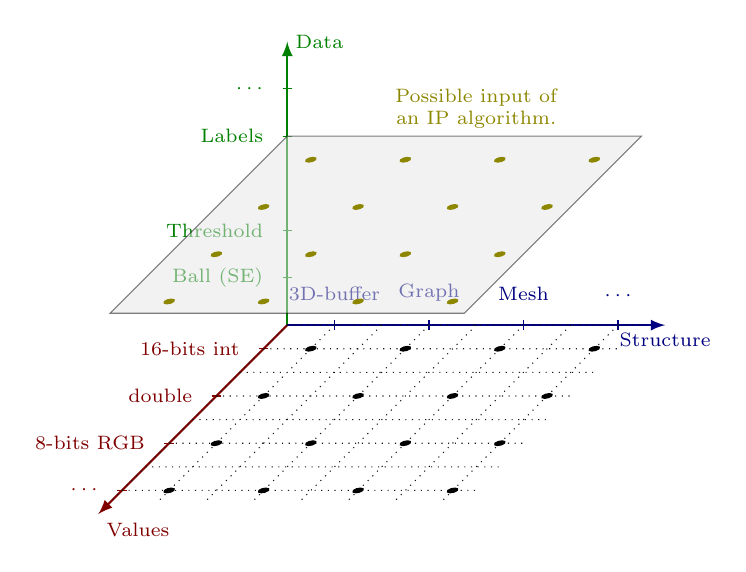
\begin{tikzpicture}[x  = {(1cm,0cm)},
    y  = {(0cm,1cm)},
    z  = {(-.5cm,-.5cm)},
    scale=.6]

  \scriptsize
  \tikzset{
    DA/.style={left=.2cm, thick,
        append after command={+(-.1,0) -- +(.1,0)}
      },
    IM/.style={above=.2cm, thick,
        append after command={+(0,-.1) -- +(0,.1)}
      },
    VA/.style={left=0cm, left=.2cm, thick,
        append after command={+(-.1,0) -- +(.1,0)}
      },
    repere/.style={thick,-latex}
  }

  % Label 1
  \draw[green!50!black,repere] (0,0,0) -- (0,6,0) node[right] {Data};
  \draw[green!50!black] (0,1,0) node[DA] {Ball (SE)};
  \draw[green!50!black] (0,2,0) node[DA] {Threshold};
  \draw[green!50!black] (0,4,0) node[DA] {Labels};
  \draw[green!50!black] (0,5,0) node[DA] {$\cdots$};

  % Label 2
  \draw[blue!50!black,repere] (0,0,0) -- (8,0,0) node[below] {Structure};
  \draw[blue!50!black] (1,0,0) node[IM] {3D-buffer};
  \draw[blue!50!black] (3,0,0) node[IM] {Graph};
  \draw[blue!50!black] (5,0,0) node[IM] {Mesh};
  \draw[blue!50!black] (7,0,0) node[IM] {$\cdots$};

  % Label 3
  \draw[red!50!black,repere] (0,0,0) -- (0,0,8) node[below right] {Values};
  \draw[red!50!black] (0,0,1) node[VA] {16-bits int};
  \draw[red!50!black] (0,0,3) node[VA] {double};
  \draw[red!50!black] (0,0,5) node[VA] {8-bits RGB};
  \draw[red!50!black] (0,0,7) node[VA] {$\cdots$};

  % Lower plane
  \begin{scope}[canvas is zx plane at y=0]
    \draw[black!90, dotted] (0,0) grid (7.5,7.5);
    \foreach \x in {1,3,5,7}
    \foreach \y in {1,3,5,7}
    \filldraw (\x,\y) circle (0.1);
  \end{scope}

  % Upper plane
  \begin{scope}[canvas is zx plane at y=4]
    \filldraw[fill=gray!20,opacity=0.5] (0,0) rectangle (7.5,7.5);
    \node[above, olive, text width=4cm, align=center] at (0,4) {
      Possible input of an IP algorithm.
    };
    \foreach \x in {1,3,5,7}
    \foreach \y in {1,3,5,7}
    \filldraw[olive] (\x,\y) circle (0.1);
  \end{scope}

\end{tikzpicture}
\end{document}


